\documentclass[a4paper,12pt]{article}
\usepackage[T1]{fontenc}
\usepackage[margin=1.9cm]{geometry}
\usepackage{graphicx}
\usepackage{subcaption}
\usepackage{xcolor}
\usepackage[hidelinks]{hyperref}
\usepackage[scaled]{helvet}
\usepackage{tocloft}
\usepackage[inline]{enumitem}
\usepackage{tabularx}
\newlist{notes}{enumerate}{1}
\setlist[notes]{label=Note \arabic*: ,leftmargin=*}
\renewcommand{\cftsecleader}{\cftdotfill{\cftdotsep}} % for parts
\renewcommand\familydefault{\sfdefault}
\title{UX Rework: Battlerite Client}
\author{Curlicue}
\date{December 6, 2018}
\begin{document}
\pagecolor{black!3}
\setlength{\parindent}{0in}

\maketitle

\tableofcontents

\newpage
\section{Introduction}
 
This is but a practice exercise with the simple goal of gettinng exposed to new problems whilst designing a product and a step into solidifying a design process that I'll be able to use in the future. The excerice will be designing a Battlerite desktop (Windows).
\begin{notes}
    \item All of the following is not in any way a critique and solely my opinion.
    \item All of the following does not take in consideration ports to other platforms.
\end{notes}

\newpage
\section{The Fundamentals}
\label{the_fundamentals}

Every decision that's made will consider 4 elements:
\begin{enumerate}[label=\textbf{\arabic*})]
    \item \textbf{Balance between relevancy and ease of accessibility.} This means finding the sweet spot for the positioning of every UI element between how much the user wants to access it and how easy it is to access in comparrison to all the other content.
    \item \textbf{Information duplication.} When information is duplicated and accessible in more than one way it introduces unecessary confusion to the user. Ensuring this doesn't happen will enable the user to memorize exactly where to go for each type of information avoiding frustration and time wasted.
    \item \textbf{Decoupling sections from each other.} Having multiple content even if of similiar nature accessible under a shared section can force the user to have to make an assumption of what will be in that section. E.g.: A section labeled "Stats" where a user can find both their performance stats, as well as tips on how to improve. This can make sense because tips on how to improve are very tightly related to a user's stats, but they can also be a standalone thing -- when a user is clicking stats they can't safely assume that tips will be there, meaning:
    \begin{enumerate*}[label=\arabic*)]
        \item it makes it more difficult to remember that the tips are accessible on the "Stats" section; and
        \item a user won't discover the tips unless they're interested in the "Stats".
    \end{enumerate*}
    \item \textbf{Upcoming content.} Ensuring there is space to add upcoming content and sections whatever they may be enables a quicker feature development process.
\end{enumerate}

\newpage
\section{Identifying Problems}

As a user, the majority of the problems I ran into were due to duplicated information, I consider myself an average type of user and I'm not conducting any type of user research so I'll go with the assumptions that these are also the issues other users have.\\
In this section I try to identify these problems, and in the following section I try to come up with solutions.
\begin{enumerate}[label=\textbf{\arabic*})]
    \item \textbf{How to start a game} -- Where to go to start playing is seperated into the \textit{Play} and \textit{Practice} sections. This can create 2 problems. \begin{itemize}
        \item It's not unreasonable for people to assume that every game mode will be listed in the \textit{Play} section, hence being left with the impression that they're exposed to every game mode in that section, while there are other game modes listed in the \textit{Practice} section.
        \item This division makes the co-op mode (VS AI) be a fit for both sections, hence making it very difficult for people to know in which one it is.
        \begin{figure}[h!]
            \centering
            \begin{subfigure}[b]{0.45\linewidth}
                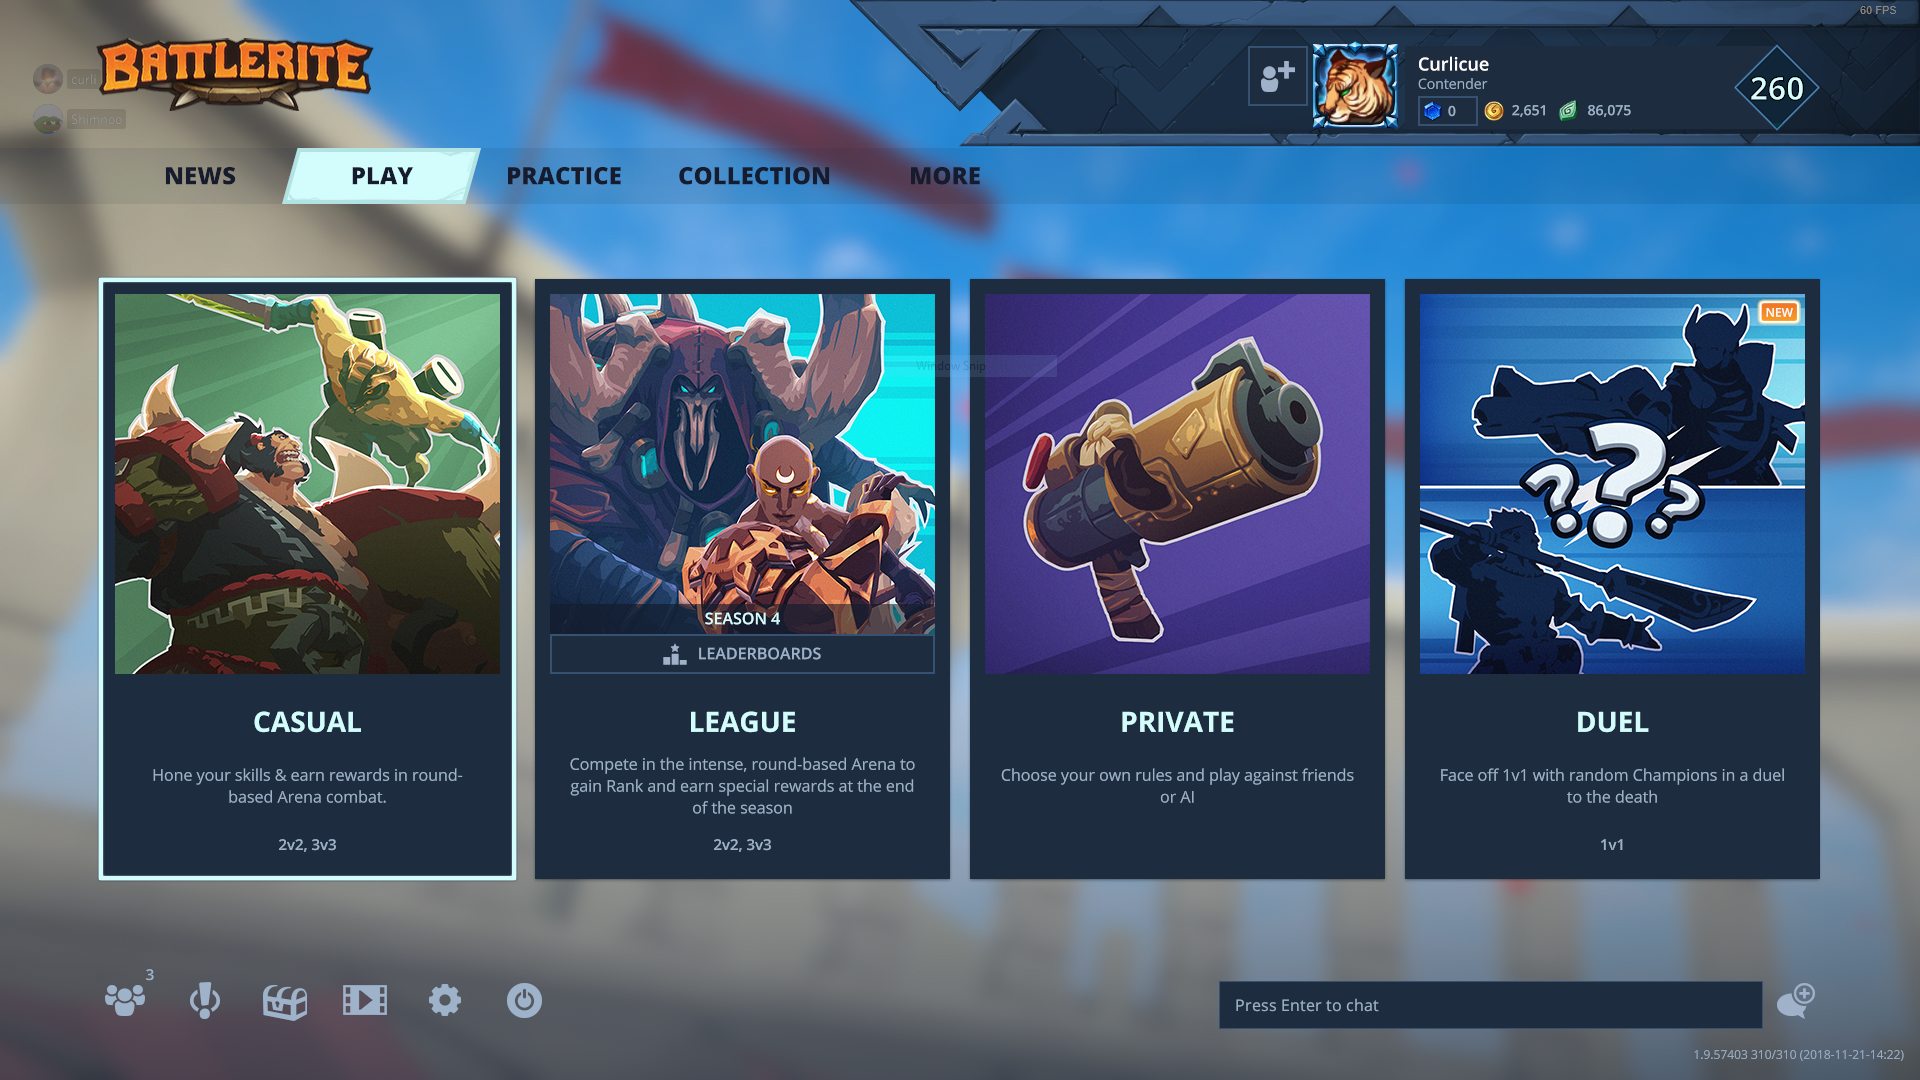
\includegraphics[width=\linewidth]{res/current/play.png}
                \caption{Play section}
            \end{subfigure}
            \begin{subfigure}[b]{0.45\linewidth}
                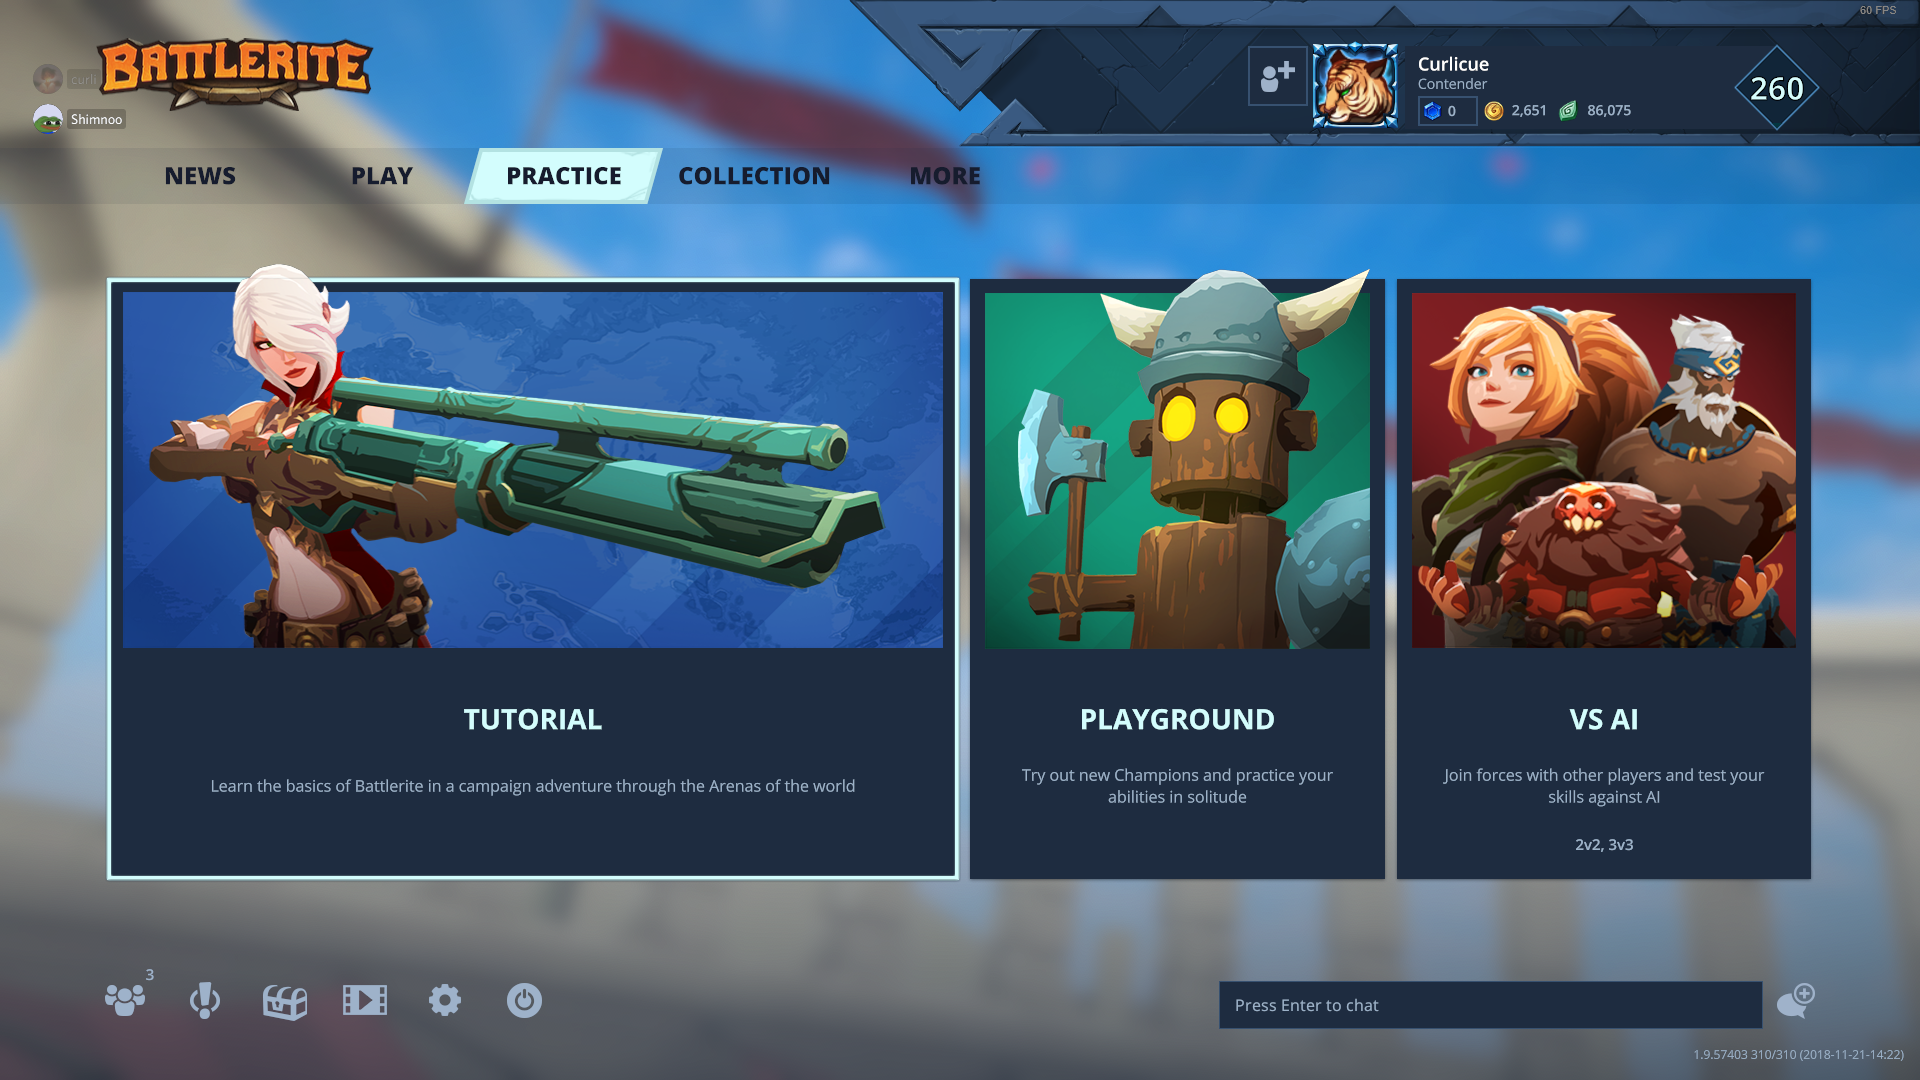
\includegraphics[width=\linewidth]{res/current/practice.png}
                \caption{Practice section}
            \end{subfigure}
            \caption{How to start a game}
            \label{fig:play_vs_practice}
        \end{figure}
    \end{itemize}
    
    \item \textbf{Collection/Profile} -- It's often seen in many applications a clash between personal information, personal content, and account settings, it can be too much information to put in one section and also difficult to seperate. In this case, the settings are well seperated from the content, but having \textit{Collection} and \textit{Profile} can introduce some confusion on where each thing is -- even though the \textit{Profile} section is focused on mostly personal stats, it's still resonable for a user to assume that actions such as changing the name, avatar and title would be done under the \textit{Profile} section.
    \begin{figure}[h!]
        \centering
        \begin{subfigure}[b]{0.45\linewidth}
            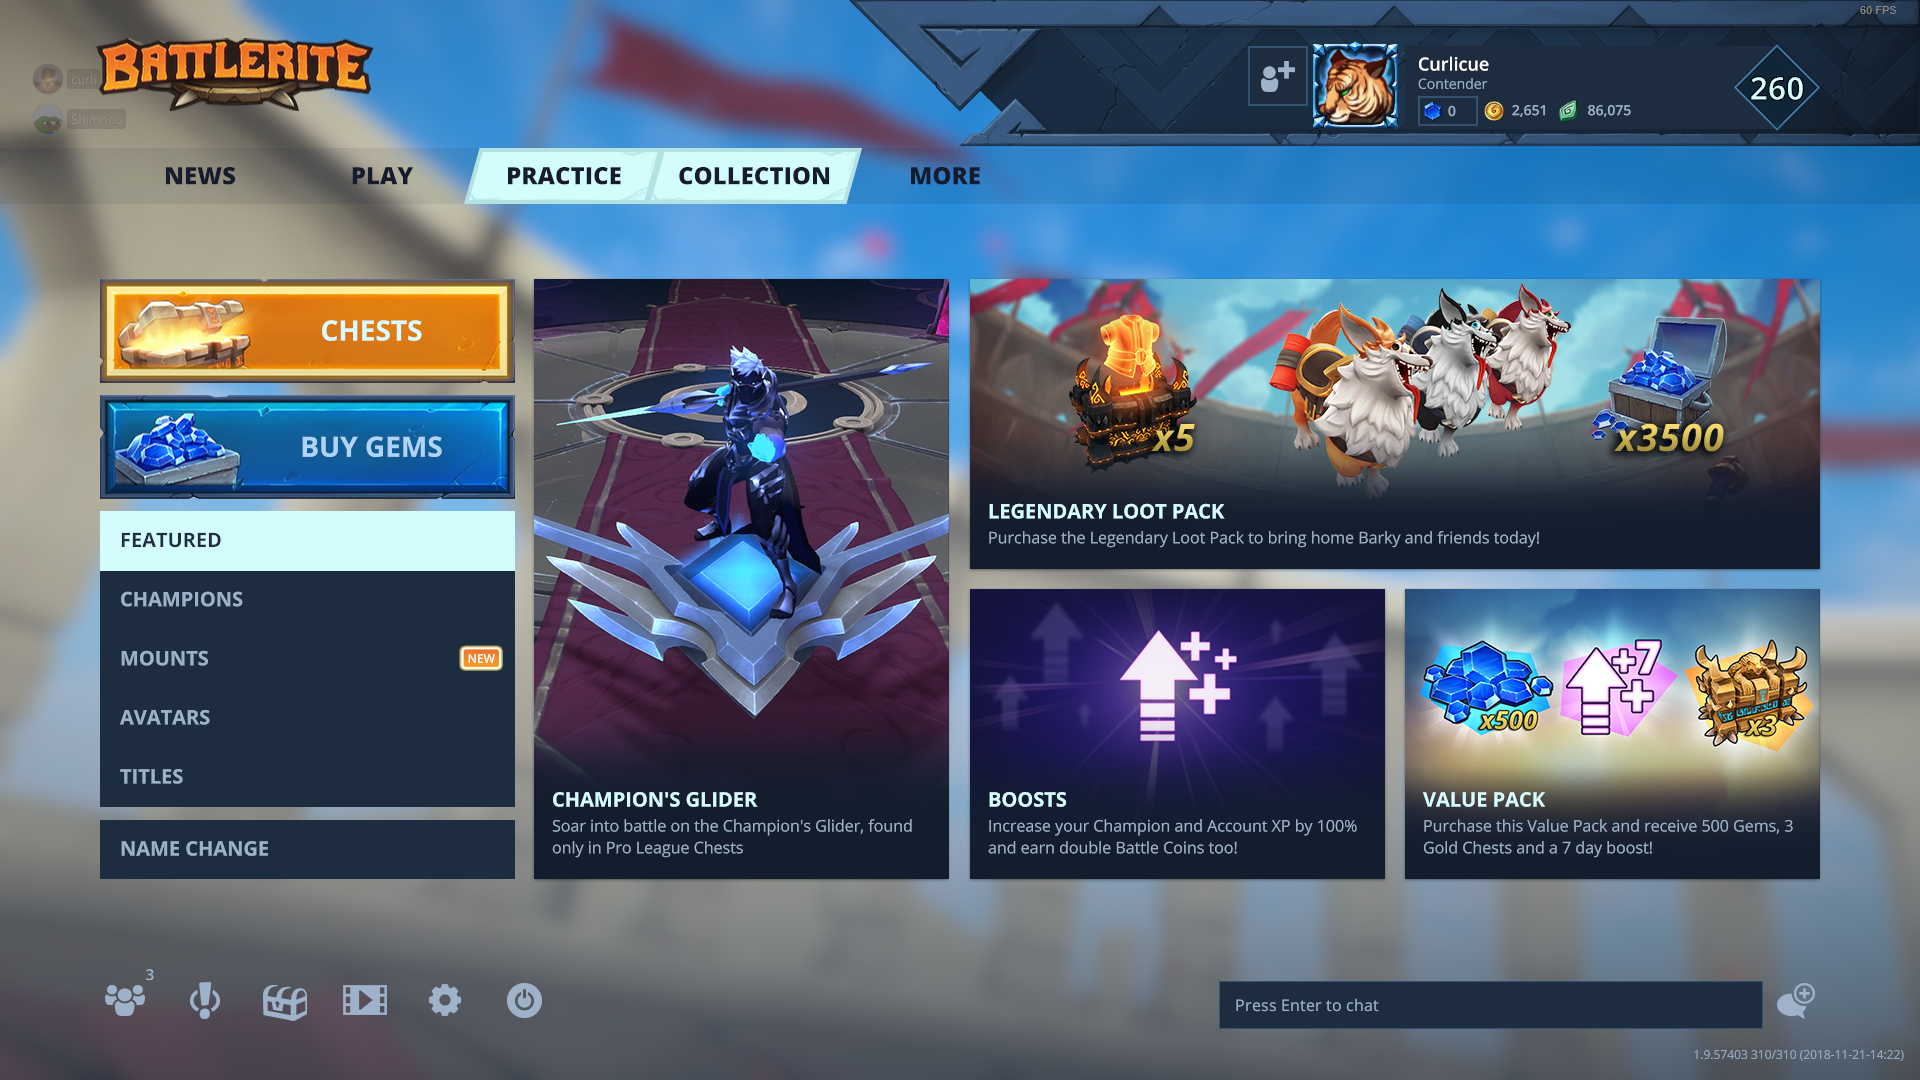
\includegraphics[width=\linewidth]{res/current/collection.png}
            \caption{Collection section}
        \end{subfigure}
        \begin{subfigure}[b]{0.45\linewidth}
            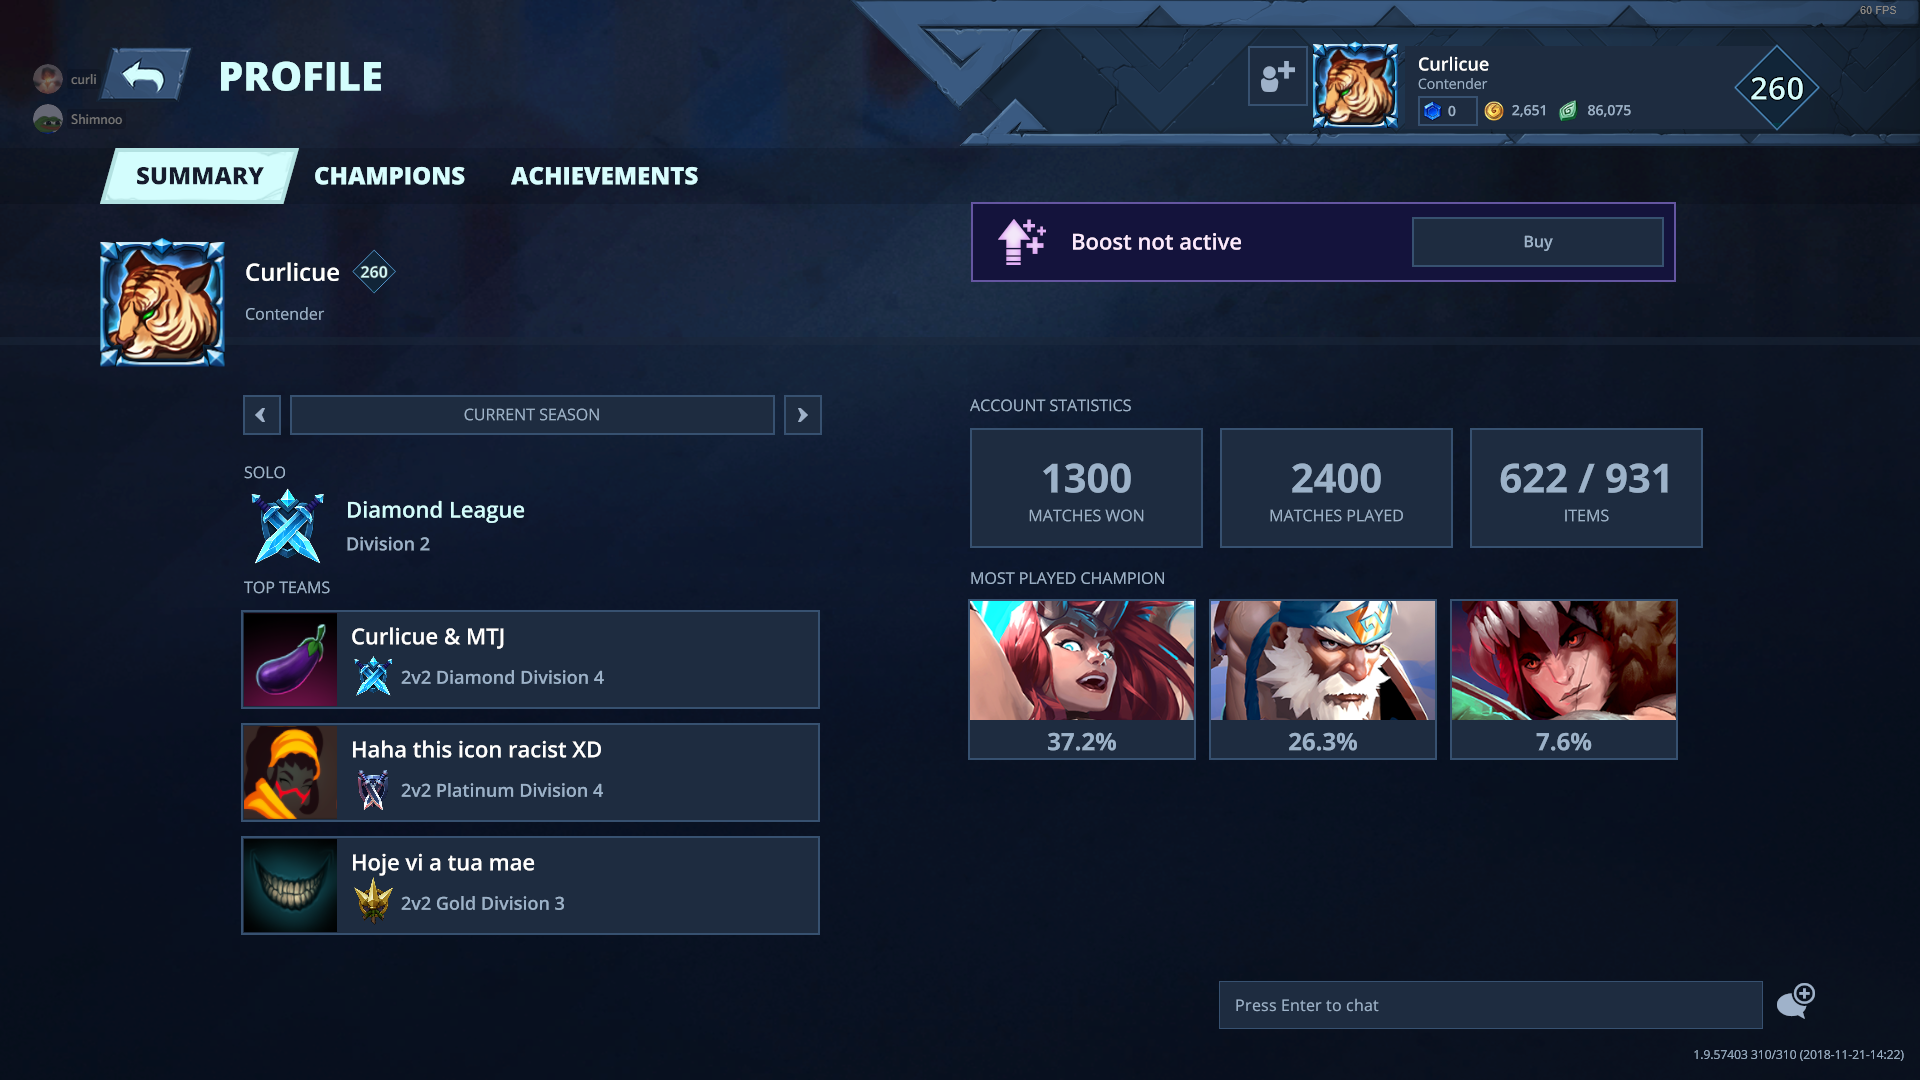
\includegraphics[width=\linewidth]{res/current/profile.png}
            \caption{Profile section}
        \end{subfigure}
        \caption{Collection and Profile sections clash}
        \label{fig:play_vs_practice}
    \end{figure}
    
    \newpage
    \item \textbf{More section} -- Having a section labeled exactly after what content it has allows a user to instantly know what to expect when clicking it, e.g. Leaderboards. Having a section labeled \textit{More} has the opposite effect -- extremly difficult for a user to know what to expect, hence memorizing what it contains and when to go there. An extra layer of complexity is also introduced by having some of the content in \textit{More} duplicated in the seondary menu at the bottom.
    \begin{figure}[h!]
        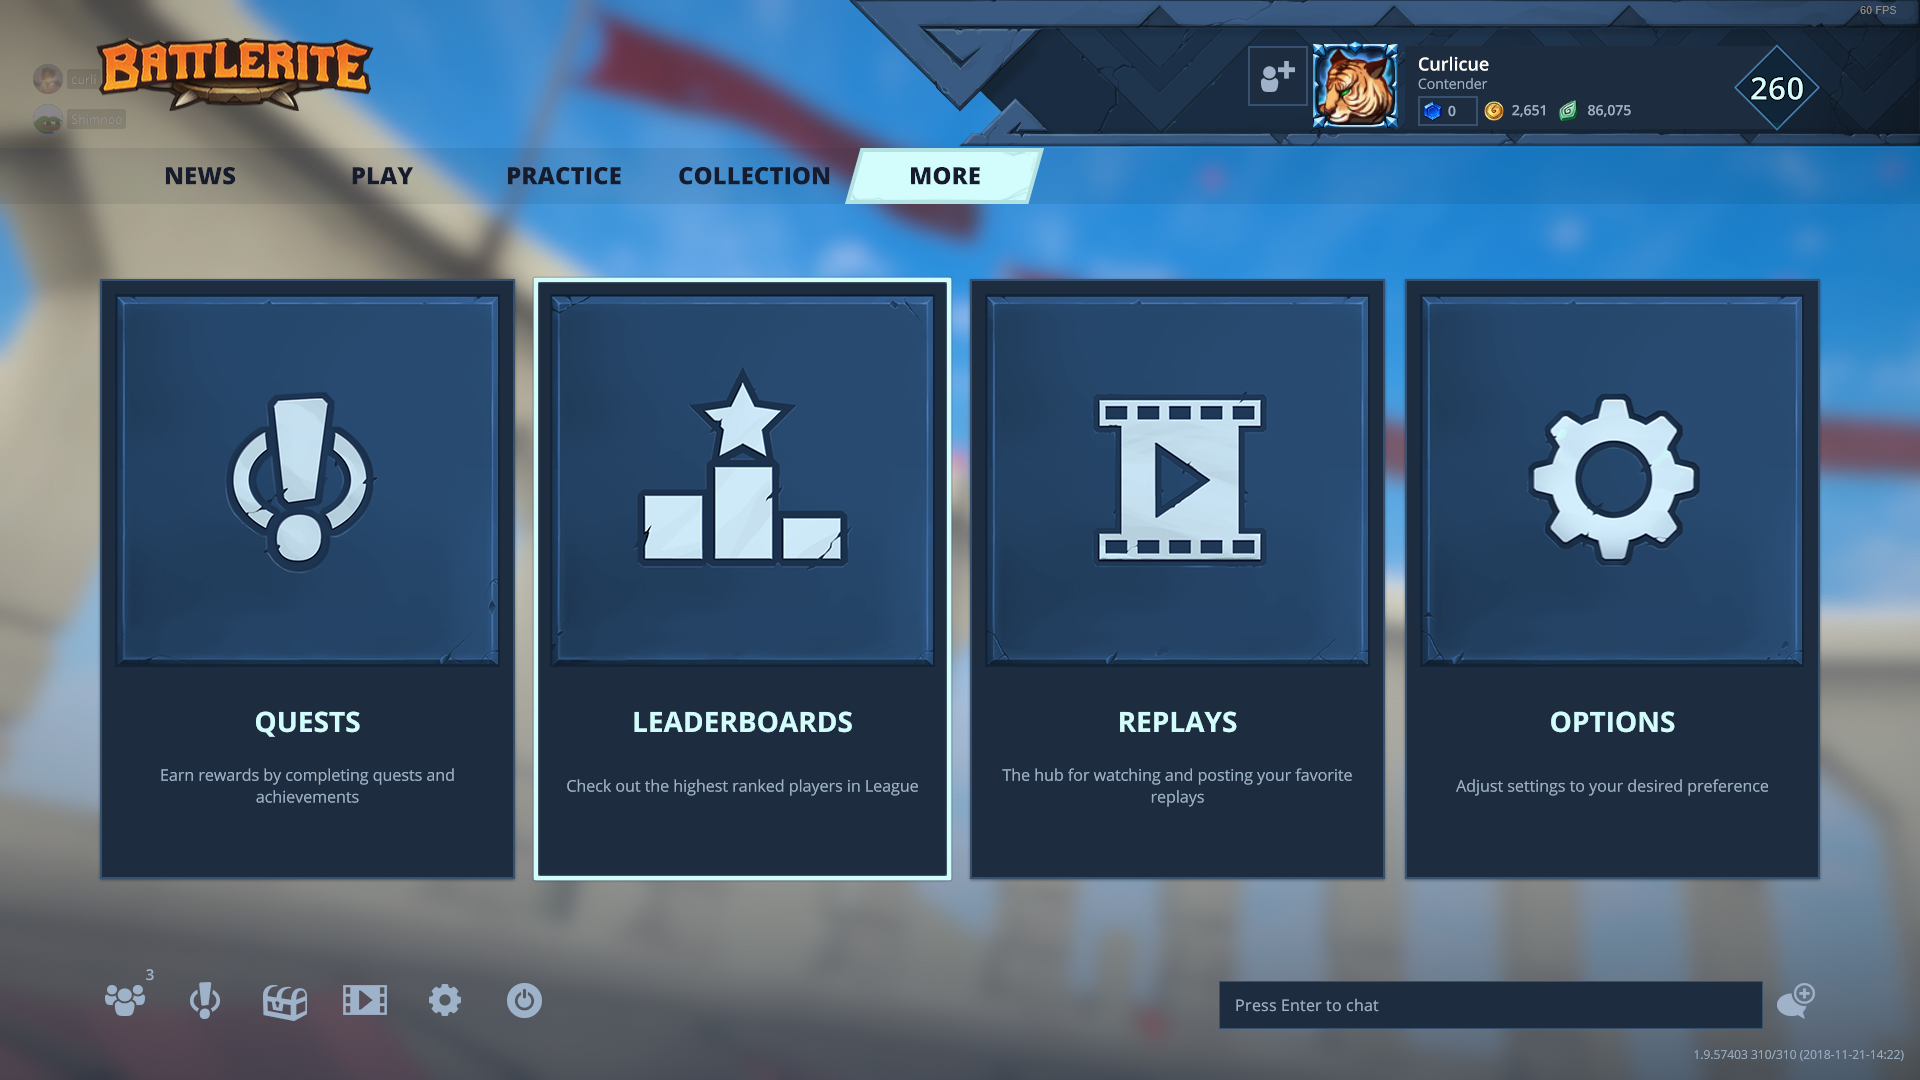
\includegraphics[width=0.45\linewidth]{res/current/more.png}
        \centering
        \caption{More section}
    \end{figure}
    
    \item \textbf{Navigation} -- As mentioned in the other points, having two navigation menus can be confusing when there isn't a clear differenciation between them. A terceary nagivation menu is also available through the Esc key that has some of the section from the secondary menu along with the Profile.
    \begin{figure}[h!]
        \centering
        \begin{subfigure}[b]{0.45\linewidth}
            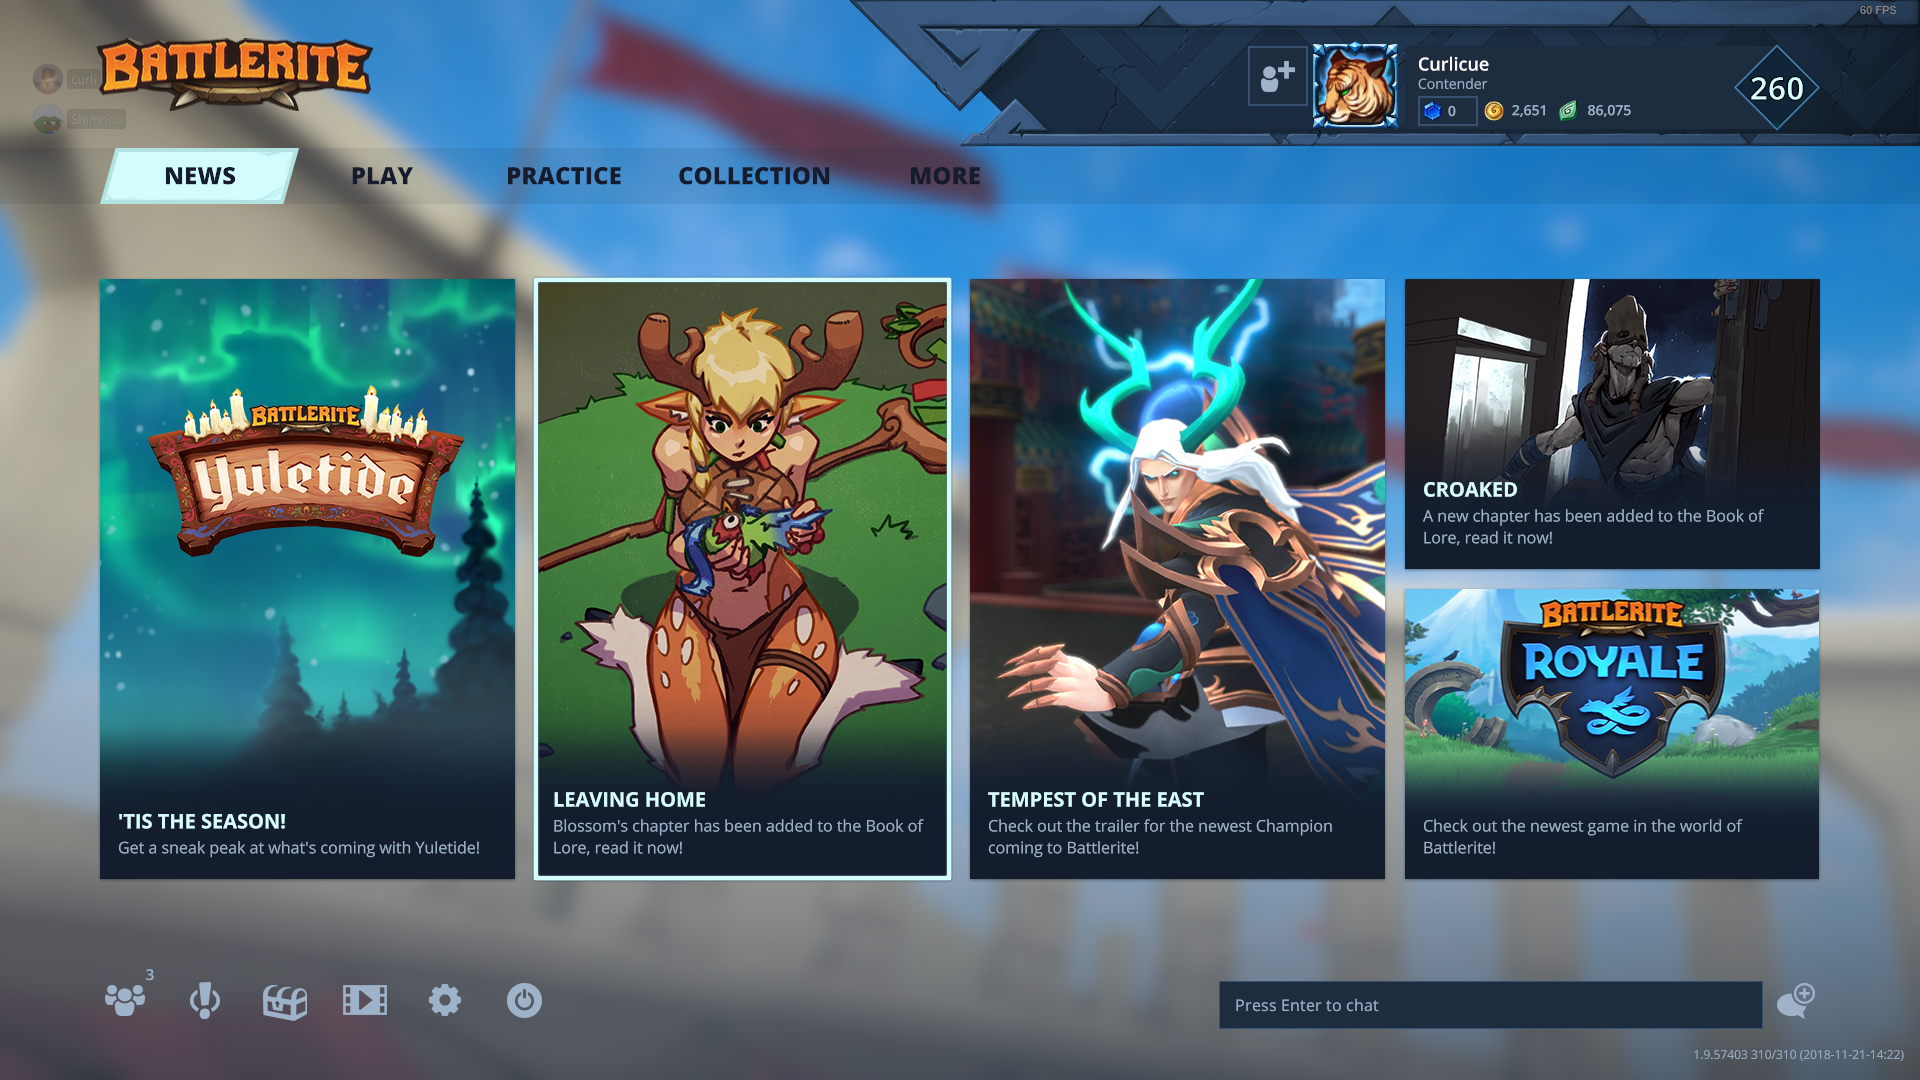
\includegraphics[width=\linewidth]{res/current/news.png}
            \caption{Main menu and secondary menu}
        \end{subfigure}
        \begin{subfigure}[b]{0.45\linewidth}
            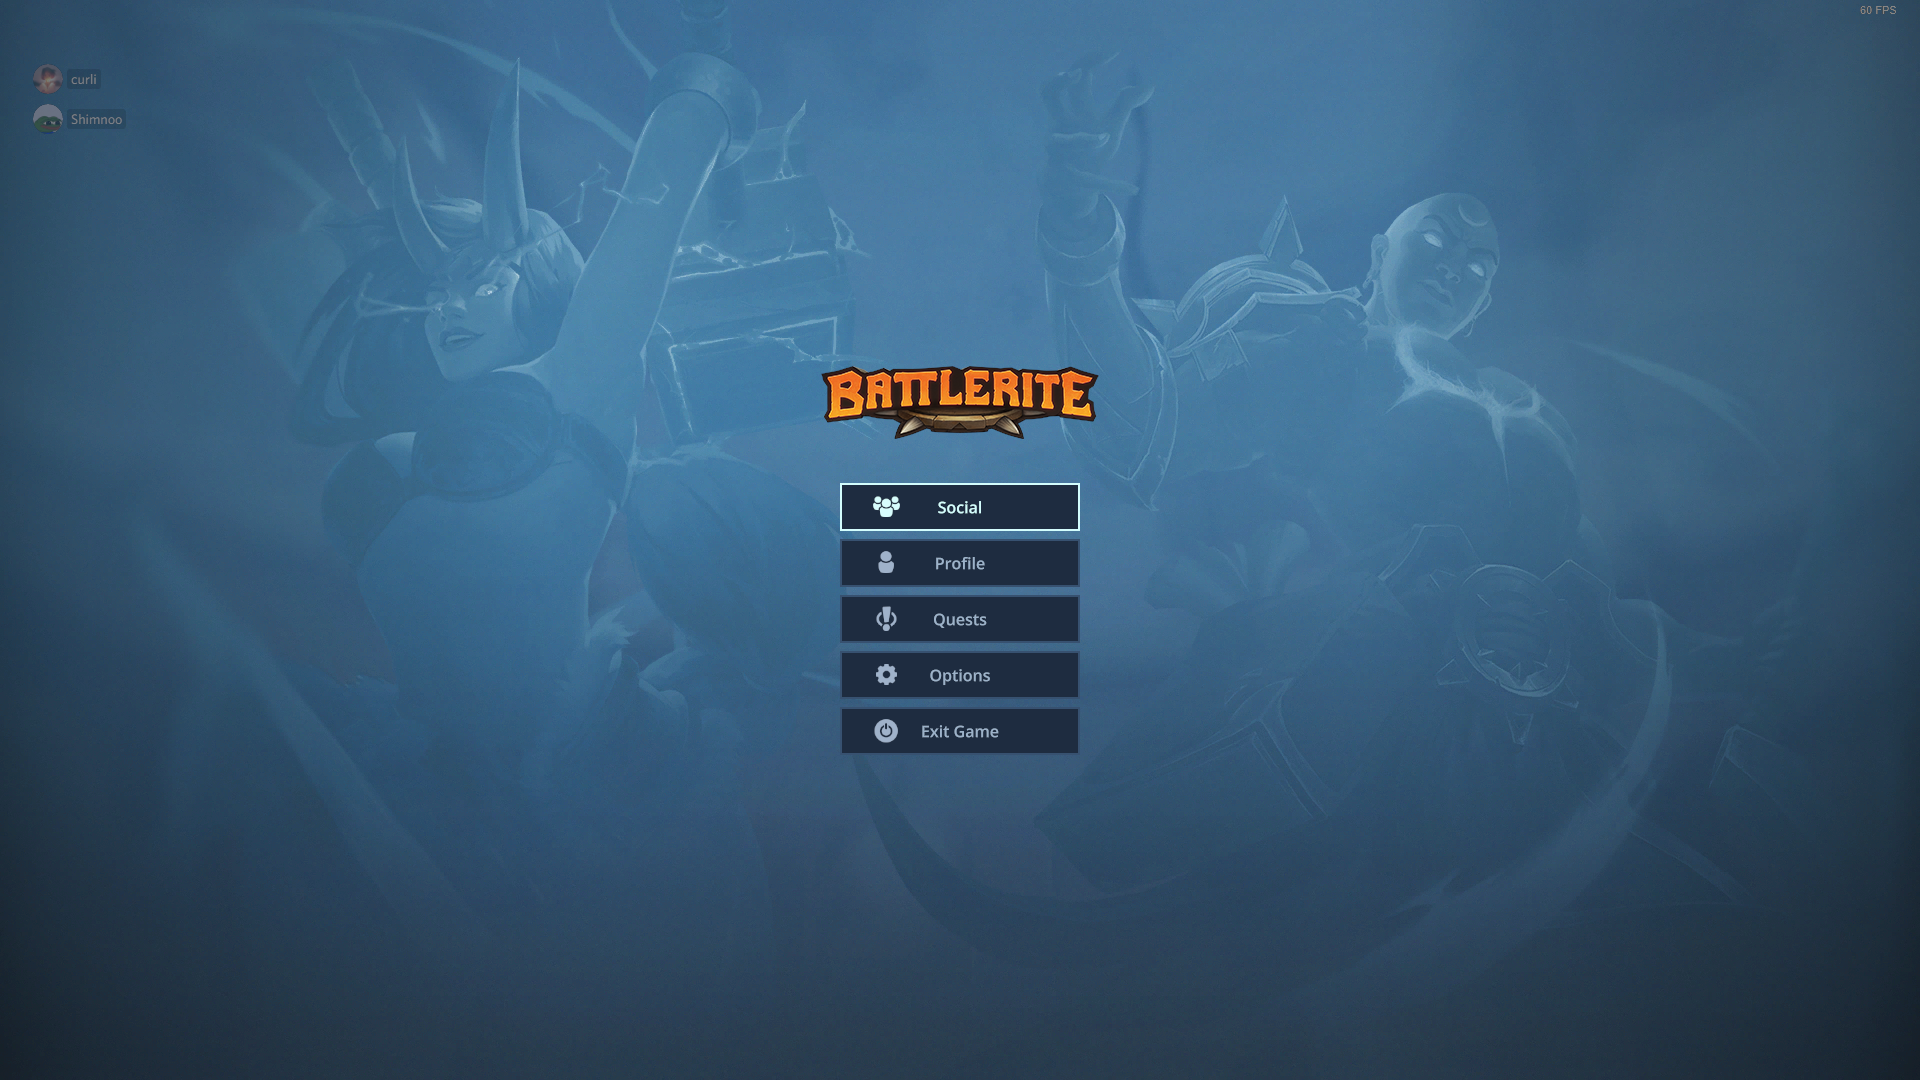
\includegraphics[width=\linewidth]{res/current/escape.png}
            \caption{Esc menu}
        \end{subfigure}
        \caption{Navigation}
        \label{fig:play_vs_practice}
    \end{figure}
    
    \item \textbf{Smaller issues} \begin{itemize}
        \item \textbf{Fullscreen client} -- impeding multi tasking while not in-game -- by utilizing the whole screen's window and by now allowing the mouse to move out of the client.
    \end{itemize}
\end{enumerate}

\newpage
\section{The Work}
I first try to divide all of information present in the client, label it and give it a relevancy rank in a way that checks all the elements in \nameref{the_fundamentals}.\\ \null \\
Then designing the experience following the divisions set above.

\def\arraystretch{1.8}
\begin{center}
    \begin{tabular}{ | p{4.3cm} | p{8.6cm} | l | }
    \hline
    \textbf{Section} 
    & \textbf{Actions / Notes}
    & \textbf{Relevancy (1-6)} 
    \\ \hline
    Play 
    & Casual, league, private, special, tutorial, playground and vs bots. 
    & 6
    \\ \hline
    News 
    & Articles, promotions, events, etc. 
    & 5
    \\ \hline
    Store 
    & Purchase champions, skins, mounts, emotes, boosts, name change, all champions pack, Legendary loot pack, Ultimate fan pack, Soundtrack and Royale game.
    & 5
    \\ \hline
    Collection 
    & See your champions, skins, emotes, loadouts and mounts. 
    & 5
    \\ \hline
    Settings 
    & 
    & 4
    \\ \hline
    Chests 
    & See the chests you own and open them. 
    & 4
    \\ \hline
    Challenges 
    & Quests, achivements and sponsors. 
    & 4
    \\ \hline
    League 
    & See your league, teams and leaderboards. 
    & 3
    \\ \hline
    Friends 
    & See who's playing and chat 
    & 3 
    \\ \hline
    Profile preview
    & Change title and avatar, see currency
    & 2
    \\ \hline
    Stats 
    & Matches played/won and champions win ratios. 
    & 2
    \\ \hline
    Replays 
    & (Current view) Trending, new, following, post, filter by player, see your posts
    & 1 
    \\ \hline
    \end{tabular}
\end{center}

\newpage
First attempt.
\begin{figure}[h!]
    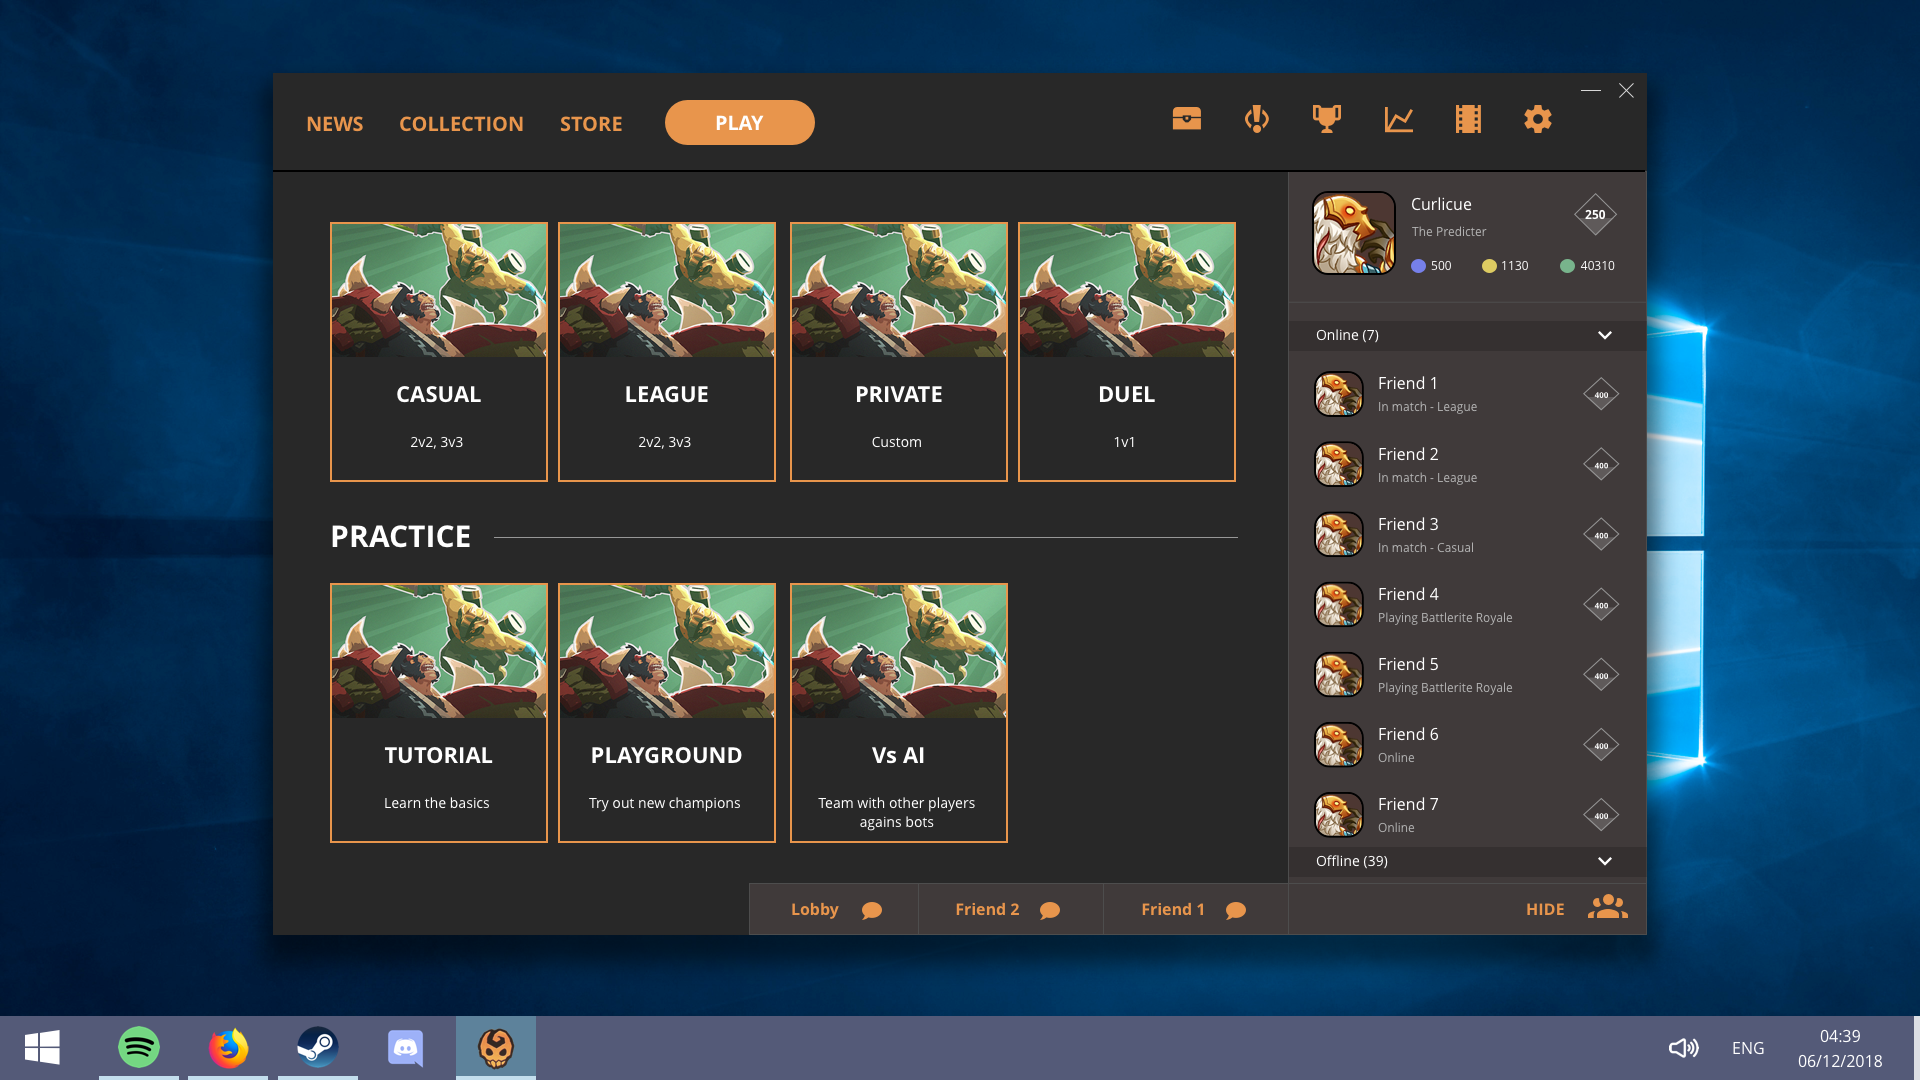
\includegraphics[width=1\linewidth]{res/play.png}
    \centering
    \caption{Play section}
\end{figure}


\end{document}
